\documentclass{article}
\usepackage{graphicx} % Required for inserting images
\usepackage[utf8]{inputenc}
\usepackage[greek,english]{babel}
\usepackage{amsmath}
\usepackage{tcolorbox} 
\usepackage{xcolor}
\usepackage{array}
\usepackage{enumitem}
\usepackage{multirow}
\usepackage{graphicx}


\renewcommand{\thesubsubsection}{\thesubsection.\alph{subsubsection}}

\title{Assignment in Numerical Analysis LaTeX}
\author{Full Name: Savvidis Theocharis 4555}
\date{10 December 2024}

\begin{document}


\maketitle

%%%%%%%%%%%%%%%%%%%%%%%%%%%%%%%%%%%%%%%%%%%%%%%%%%%%%%%%%%%%%%%%%%%%%
\section{First Exercise}

\subsection{Bisection method}

After testing the final code 5 times with different values of the lower (a) and upper (b) bounds the results are the following :
\begin{enumerate}
\begin{tcolorbox}[colback=blue!10, colframe=gray!80, width=\textwidth, sharp corners]

\item \textbf{For root = -1.1976237}
\begin{center}
    a = -2 \\
    b = -1 \\
    Iterations: 23
    \vspace{0.3cm}
\end{center}
\begin{center}
    a = -1.5 \\
    b = -1 \\
    Iterations: 22
    \vspace{0.3cm}
\end{center}
\begin{center}
    a = -1.2 \\
    b = -1 \\
    Iterations: 20
    \vspace{0.3cm}
\end{center}
\begin{center}
    a = -1.19 \\
    b = -1.2 \\
    Iterations: 16
    \vspace{0.3cm}
\end{center}
\begin{center}
    a = -1.197 \\
    b = -1.198 \\
    Iterations: 13
    \vspace{0.2cm}
\end{center}
\end{tcolorbox}
\begin{tcolorbox}[colback=blue!10, colframe=gray!80, width=\textwidth, sharp corners]

\item \textbf{For root = 1.5301335}
\begin{center}
    a = -1 \\
    b = 2 \\
    Iterations: 24
    \vspace{0.3cm}
\end{center}
\begin{center}
    a = 0.5 \\
    b = 2 \\
    Iterations: 23
    \vspace{0.3cm}
\end{center}
\begin{center}
    a = 1.4 \\
    b = 1.6 \\
    Iterations: 20
    \vspace{0.3cm}
\end{center}
\begin{center}
    a = 1.5 \\
    b = 1.6 \\
    Iterations: 19
    \vspace{0.3cm}
\end{center}
\newpage
\begin{center}
    a = 1.53 \\
    b = 1.531 \\
    Iterations: 13
    \vspace{0.3cm}
\end{center}


\item \textbf{For root = 0}
\begin{center}
    a = -1.4\\
    b = 1.4 \\
    Iterations: 1
    \vspace{0.3cm}
\end{center}
\begin{center}
    a = -1.3 \\
    b = 1.3 \\
    Iterations: 1
    \vspace{0.3cm}
\end{center}
\begin{center}
    a = -1.2  \\
    b = 1.2 \\
    Iterations: 1
    \vspace{0.3cm}
\end{center}
\begin{center}
    a = -1.25 \\
    b = 1.25 \\
    Iterations: 1
    \vspace{0.3cm}
\end{center}
\begin{center}
    a = -1.199 \\
    b = 1.199 \\
    Iterations: 1
    \vspace{0.3cm}
\end{center}


\end{tcolorbox}
\end{enumerate}
\begin{tcolorbox}[colback=gray!10, colframe=gray!80, width=\textwidth, sharp corners]
    \centering 
    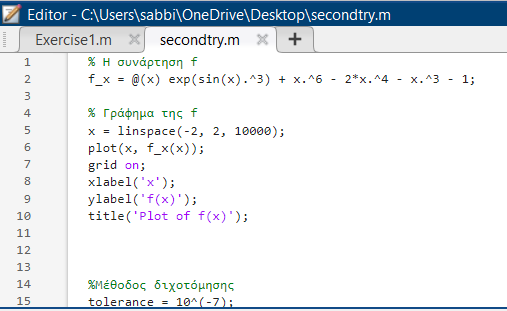
\includegraphics[width=0.5\textwidth,height=0.198\textheight]{Plot1Code.png} 

    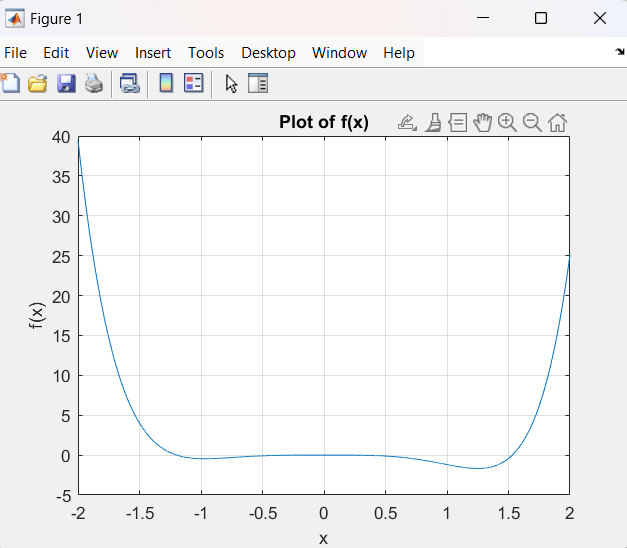
\includegraphics[width=0.6\textwidth,height=0.22\textheight]{Plot1.png}
    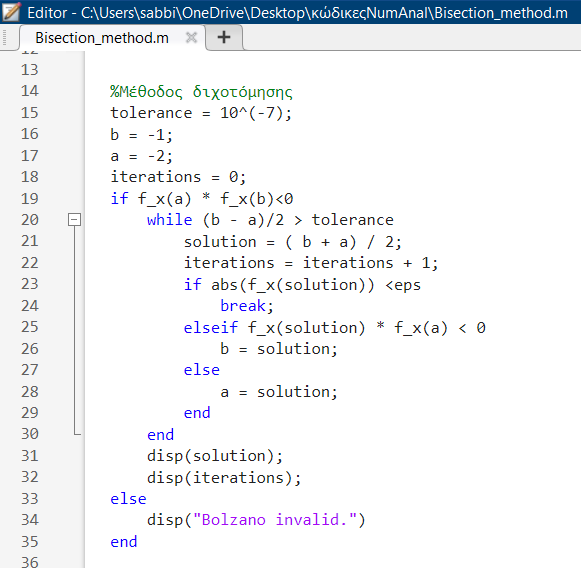
\includegraphics[width=0.5\textwidth,height=0.24\textheight]{Bisection.png}

    \vspace{0.5cm} 
    
    \vspace{0.5cm}
    \small\textit{Note: The above code was implemented without the assistance of language model.}
\end{tcolorbox}

\subsection{Newton-Raphson method}

\begin{tcolorbox}[colback=blue!10, colframe=gray!80, width=\textwidth, sharp corners]

\begin{enumerate}

\item For root = -1.1976237
\begin{center}

    $x_{n-1}$ = -2\\
    Iterations: 7\\
    \vspace{0.3cm}
    $x_{n-1}$ = -1.7\\
    Iterations: 5\\
    \vspace{0.3cm}
    $x_{n-1}$ = 1.3\\
    Iterations: 4\\
    \vspace{0.3cm}
    $x_{n-1}$ = -1.2\\
    Iterations: 2\\
    \vspace{0.3cm}
    $x_{n-1}$ = -1\\
    Iterations: 9\\
      
\end{center}

\item For root = 0
\begin{center}
    \textit{The initialization $x_{n-1}$  = 0 is itself leading to 0 ($f(0)=0 $) and it cannot be approached by other initializations except those being 5 or more precision digits close to 0 }
\end{center}
\item For root = 1.5301335
\begin{center}

    $x_{n-1}$ = 1.3\\
    Iterations: 8\\
    \vspace{0.3cm}
    $x_{n-1}$ = 1.5\\
    Iterations: 3\\
    \vspace{0.3cm}
    $x_{n-1}$ = 1.6\\
    Iterations: 4\\
    \vspace{0.3cm}
    $x_{n-1}$ = 1.8\\
    Iterations: 5\\
    \vspace{0.3cm}
    $x_{n-1}$ = 1.9\\
    Iterations: 6\\
      
\end{center}




\end{enumerate}
\end{tcolorbox}
\begin{tcolorbox}[colback=gray!10, colframe=gray!80, width=\textwidth, sharp corners]
    \centering 
    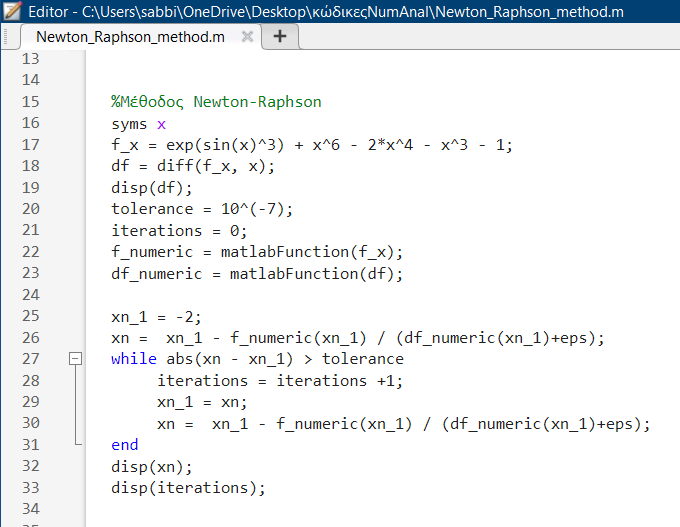
\includegraphics[width=0.5\textwidth,height=0.2\textheight]{NewtonRaphson.png} 

    \vspace{0.5cm} 
    
    \small\textit{Note: Code displaying the Newton-Raphson method. No language model was used to create the code .}
\end{tcolorbox}

 \begin{itemize}

    \item In our scenario where seven precision digits are needed, we observe quadratic convergence after finding one precision digit, three or less other iterations are needed to approach our root with 7 precision digits. That is because after finding the first precision digit then the $error$ almost becomes squared in each next iteration. That way after:
    \begin{itemize}
        \item \textbf{one iteration} we find \textbf{2 precision digits}
        \item \textbf{two iterations} we find \textbf{4 precision digits}
        \item \textbf{three iterations} we find \textbf{8 precision digits} (we have reached the required 7 precision digits)
    \end{itemize}


\begin{tcolorbox}[colback=gray!10, colframe=gray!80, width=\textwidth, sharp corners]
    \centering 
    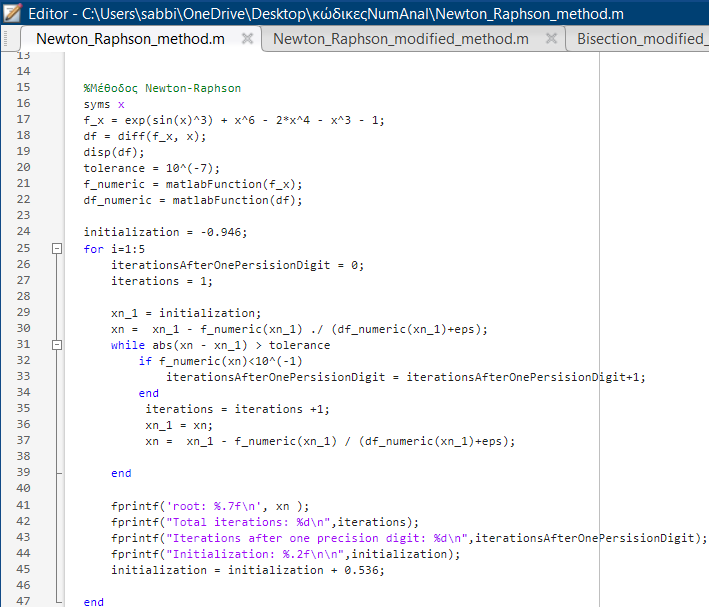
\includegraphics[width=0.5\textwidth,height=0.3\textheight]{CodeQuadraticConvergence.png} 

    \vspace{0.5cm} 
    
    \small\textit{Note: The code used for testing Quadratic convergence for all of the roots.}
\end{tcolorbox}
    
    
    \item After experimentation with a variety of values, the method seems to \textbf{not} exhibit \textbf{quadratic convergence} for the interval \textbf{[-0.95, 1.22]} (approximation), where the derivative of $f$ is approaching $0$ and in which the iterations needed to approach the root 0 are not bounded by a quadratic decrease of error but the error follows a linear decrease as it can be seen in the table below.
    \begin{tcolorbox}[colback=gray!10, colframe=gray!80, width=\textwidth, sharp corners]
    \centering 
    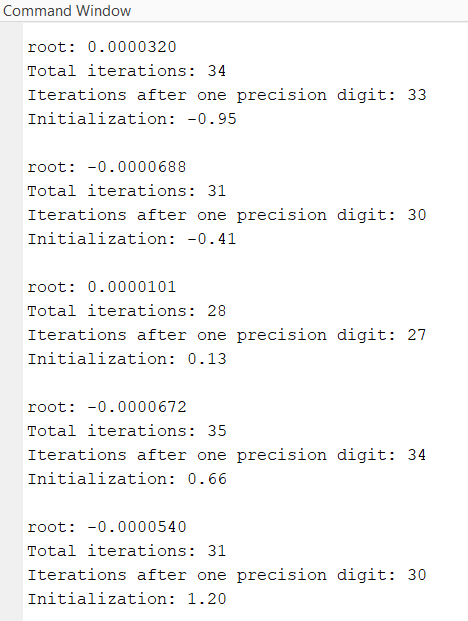
\includegraphics[width=0.5\textwidth,height=0.3\textheight]{NoQuadConvergence.png} 

    \vspace{0.5cm} 
    
    \small\textit{Note: Method does \textbf{not} converge quadratically for root 0 .}
\end{tcolorbox}

    \item For the other two intervals \textbf{(-2, -0.95)} and \textbf{(1.22, 2)} the method converges quadratically for the roots \textbf{-1.1976237 }and\textbf{ 1.5301335} correspondingly , as the iterations needed to approach a 7 digit precision root after finding the first digit of precision are less or equal to 3. The code follows similar structure to the already displayed one and the  results of the experimentation are shown below:

    \begin{tcolorbox}[colback=gray!10, colframe=gray!80, sharp corners]
    \centering
    \begin{minipage}[t]{0.48\textwidth}
        \centering
        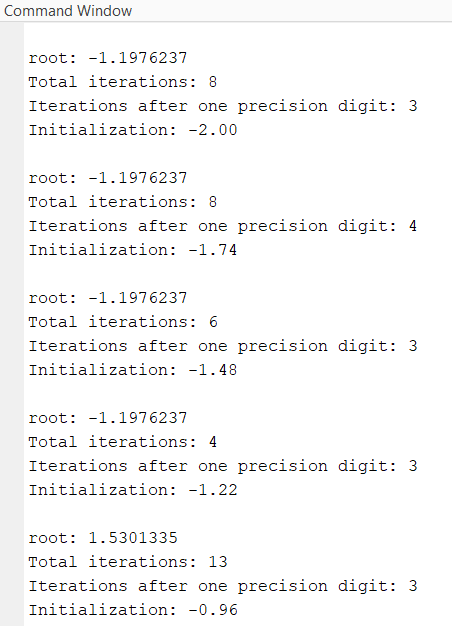
\includegraphics[width=\textwidth, height=0.25\textheight]{Root_1.19QuadraticConvergence.png}
    \end{minipage}
    \hfill
    \begin{minipage}[t]{0.48\textwidth}
        \centering
        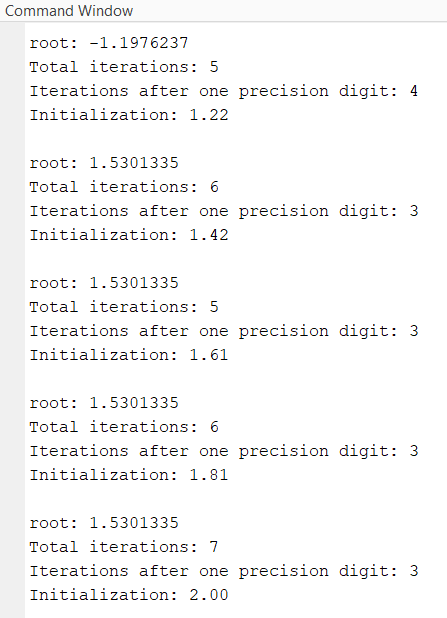
\includegraphics[width=\textwidth, height=0.25\textheight]{Root1.53QuadraticConvergence.png}
    \end{minipage}

    \vspace{0.5cm}
    
    \small\textit{Note: Method converges quadratically for roots -1.1976237 and 1.5301335.}
\end{tcolorbox}

\end{itemize}



\subsection{Secant method}
\begin{tcolorbox}[colback=blue!10, colframe=gray!80, width=\textwidth, sharp corners]

\begin{enumerate}

\item For root = -1.1976237
\begin{center}

    $x_{n-1}$ =-1  and $x_{n-2} = -2 $\\
    Iterations: 14 \\
    \vspace{0.3cm}
    $x_{n-1}$ =-1.2  and $x_{n-2} =-2  $\\
    Iterations:  4 \\
    \vspace{0.3cm}
    $x_{n-1}$ =-1.2  and $x_{n-2} =-1.5  $\\
    Iterations: 3 \\
    \vspace{0.3cm}
    $x_{n-1}$ = -1.1  and $x_{n-2} = 2  $\\
    Iterations: 8  \\
    \vspace{0.3cm}
    $x_{n-1}$ = 2 and $x_{n-2} = -1.1  $\\
    Iterations: 12 \\
      
\end{center}
\item For root = 0
\begin{center}

    $x_{n-1}$ =-1  and $x_{n-2} = 0.2 $\\
    Iterations: 49 \\
    \vspace{0.3cm}
    $x_{n-1}$ = -1  and $x_{n-2} =2  $\\
    Iterations: 60 \\
    \vspace{0.3cm}
    $x_{n-1}$ = -0.5 and $x_{n-2} = 0.5 $\\
    Iterations: 53 \\
    \vspace{0.3cm}
    $x_{n-1}$ = -0.01  and $x_{n-2} = 0.01 $\\
    Iterations: 3 \\
    \vspace{0.3cm}
    $x_{n-1}$ = -0.005 and $x_{n-2} =0.005  $\\
    Iterations: 3 \\
      
\end{center}
\item For root = 1.5301335
\begin{center}

    $x_{n-1}=1.4$   and $x_{n-2} = 1.6 $\\
    Iterations: 6 \\
    \vspace{0.3cm}
    $x_{n-1}= 1.6$   and $x_{n-2} = 1.4  $\\
    Iterations: 5 \\
    \vspace{0.3cm}
    $x_{n-1}= 1.52$   and $x_{n-2} = 1.53 $\\
    Iterations: 3 \\
    \vspace{0.3cm}
    $x_{n-1}=1.54$   and $x_{n-2} = 1.53 $\\
    Iterations: 3 \\
    \vspace{0.3cm}
    $x_{n-1}=1.53$   and $x_{n-2} = 1.54 $\\
    Iterations: 2 \\
      
\end{center}

\end{enumerate}
\end{tcolorbox}


\begin{tcolorbox}[colback=gray!10, colframe=gray!80, width=\textwidth, sharp corners]
    \centering 
    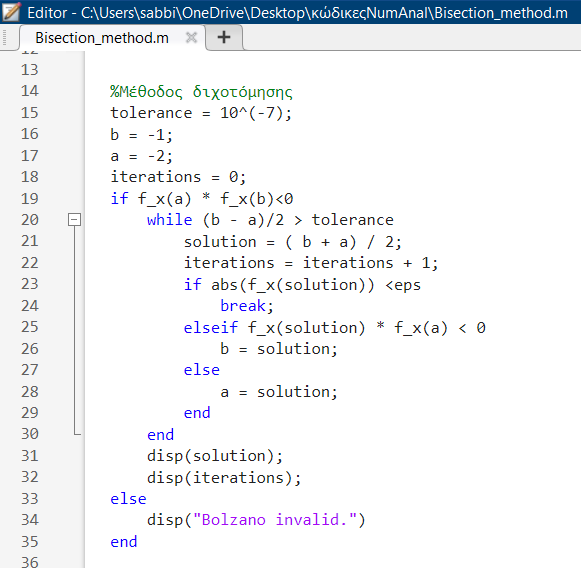
\includegraphics[width=0.55\textwidth,height=0.21\textheight]{Bisection.png} 
    
    \vspace{0.5cm}
    \small\textit{Note: The above code was implemented without the assistance of language model.}
\end{tcolorbox}

    \vspace{0.5cm} 

\section{Second Exercise}

The graph of the given function was created using the same code used for the previous one, only with changing the function.

\begin{tcolorbox}[colback=gray!10, colframe=gray!80, width=\textwidth, sharp corners]
    \centering 
    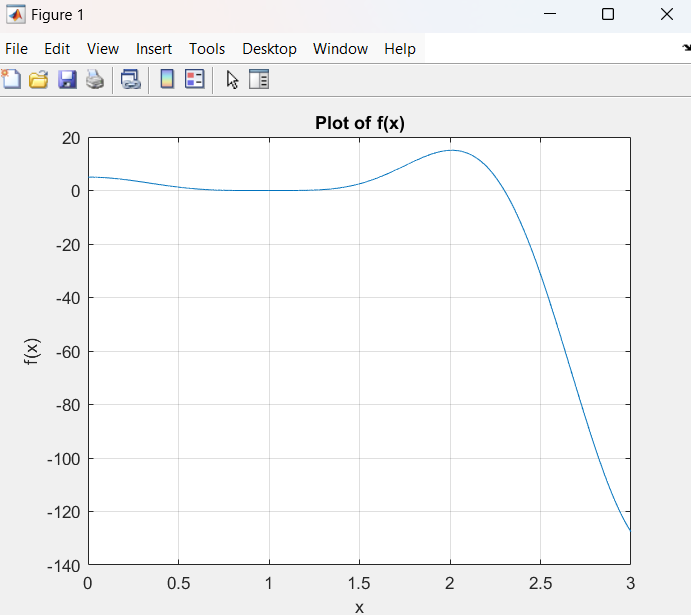
\includegraphics[width=0.8\textwidth,height=0.3\textheight]{Plot2.png} 


    \vspace{0.5cm} 
    \small\textit{Note: The graph of the given function.}
    
    
\end{tcolorbox}
    \vspace{1cm} 

Chat GPT language model was used in the second exercise \textbf{only for verifying the number of solutions} in the interval [0,3] of the given function. The following code was used:
\begin{tcolorbox}[colback=gray!10, colframe=gray!80, width=\textwidth, sharp corners]
    \centering 
    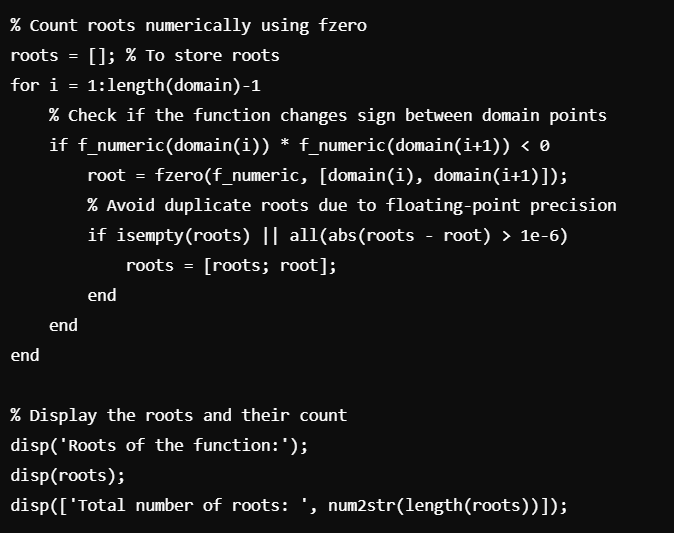
\includegraphics[width=0.8\textwidth,height=0.3\textheight]{GPTSolutionCount.png} 


    \vspace{0.5cm} 
    
\end{tcolorbox}


\vspace{0.7cm}
\subsection{Modified Newton-Raphson method}
\subsubsection{}

\begin{tcolorbox}[colback=blue!10, colframe=gray!80, width=\textwidth, sharp corners]
\begin{enumerate}
\item For $x_{n-1}$ = 0.8
\begin{center}
   \textbf{ root = 0.8410686} \\
    Iterations: 5
\end{center}
\item For $x_{n-1}$ = 2.5
\begin{center}
    \textbf{root = 2.3005239} \\
    Iterations: 5
\end{center}
\item For $x_{n-1}$ = 1.05
\begin{center}
    \textbf{root = 1.0472017} \\
    Iterations: 16
\end{center}



\end{enumerate}
\end{tcolorbox}

\begin{tcolorbox}[colback=gray!10, colframe=gray!80, width=\textwidth, sharp corners]
    \centering 
    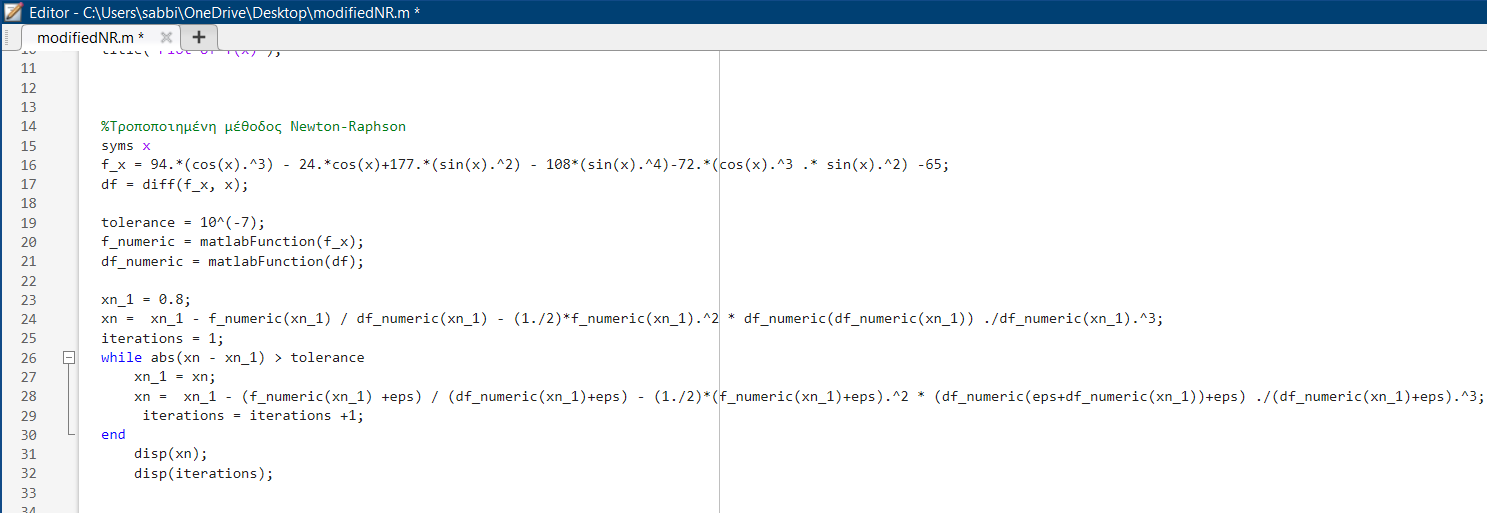
\includegraphics[width=1\textwidth,height=0.4\textheight]{NewtonRaphsonModified.png} 


    \vspace{0.5cm} 
    
    
    \small\textit{Note: The above code was implemented without the assistance of language model.}
\end{tcolorbox}

\vspace{0.7cm}
\subsection{Modified Bisection method}
\subsubsection{}

\begin{tcolorbox}[colback=blue!10, colframe=gray!80, width=\textwidth, sharp corners]
\begin{enumerate}
\item For a = 2 and b = 2.35
\begin{center}
    \textbf{root = 2.3005240} \\
    Iterations: 21
\end{center}
\item For a = 0.99 and b = 1.5
\begin{center}
    \textbf{root = 1.0471905} \\
    Iterations: 20
\end{center}
\item For a = 0.3 and b = 0.85
\begin{center}
    \textbf{root = 0.8410687} \\
    Iterations: 18
\end{center}



\end{enumerate}
\end{tcolorbox}



\begin{tcolorbox}[colback=gray!10, colframe=gray!80, width=\textwidth, sharp corners]
    \centering 
    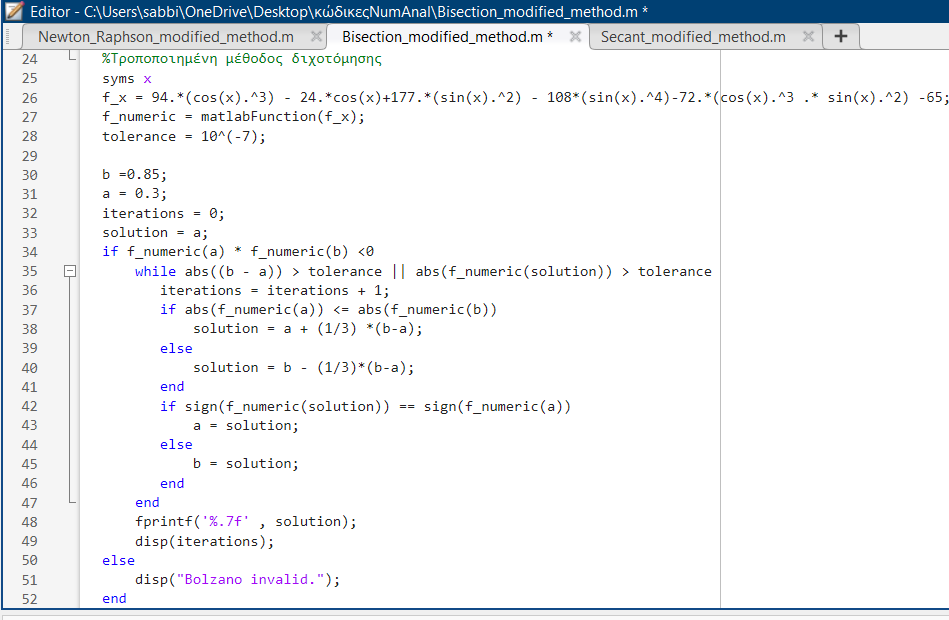
\includegraphics[width=0.8\textwidth,height=0.3\textheight]{BisectionModified.png} 


    \vspace{0.5cm} 
    
    
    \small\textit{Note: The above code was implemented without the assistance of language model.}
\end{tcolorbox}
\vspace{0.6cm}

\subsubsection{}
After adding a loop that iterates 20 times in the bisection modified method the result supports that the algorithm converges in a different number of iterations. Two experiments were conducted leading to the following results.
\vspace{0.3cm}
\begin{tcolorbox}[colback=gray!10, colframe=gray!80, width=\textwidth, sharp corners]
    \centering 
    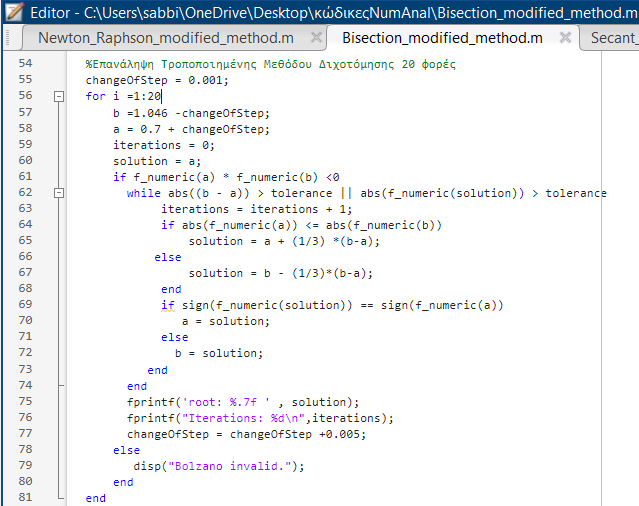
\includegraphics[width=0.8\textwidth,height=0.3\textheight]{BisectionModified20Times.png} 

    \vspace{0.2cm} 
    
    \small\textit{Note: The above code was implemented without the assistance of language model.}
\end{tcolorbox}



In the first experimentation , for $\textbf{root = 0.8410687}$ , a change \textbf{step} of \textbf{0.001} was used (in order to insure different initialization a was increased by that step and b was decreased by the same step).
\vspace{0.2cm}
\begin{tcolorbox}[colback=gray!10, colframe=gray!80, width=\textwidth, sharp corners]
    \centering 
    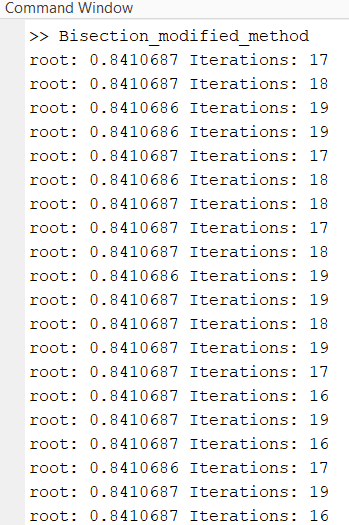
\includegraphics[width=0.6\textwidth,height=0.4\textheight]{Results20Times1.png} 


    \vspace{0.2cm} 
    
    
    \small\textit{Note: The algorithm seems to converge for a different numbers of iterations.}
\end{tcolorbox}
\vspace{0.5cm}

In the second experimentation , for $\textbf{root = 2.3005240}$ , a change \textbf{step} of \textbf{0.01} was used (in order to insure different initialization, a was increased by that step and b was decreased by the same step).
\vspace{0.2cm}
\begin{tcolorbox}[colback=gray!10, colframe=gray!80, width=\textwidth, sharp corners]
    \centering 
    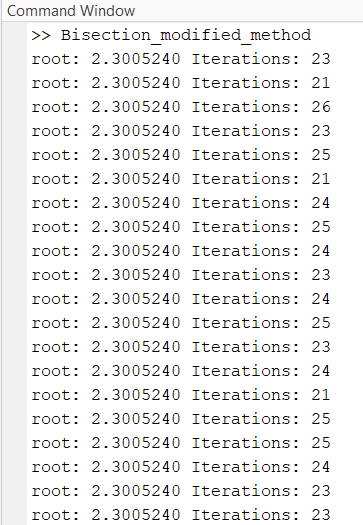
\includegraphics[width=0.6\textwidth,height=0.4\textheight]{Results20Times2.png} 


    \vspace{0.1cm} 
    
    
    \small\textit{Note: The algorithm seems to converge for a different numbers of iterations.}
\end{tcolorbox}





\subsection{Modified Secant method}
\subsubsection{}

\begin{tcolorbox}[colback=blue!10, colframe=gray!80, width=\textwidth, sharp corners]
\begin{enumerate}
\item For $x_{n}=0.8 $ and $x_{n+1}= 1.7$ and $x_{n+2}= 2.8 $ 
\begin{center}
   \textbf{ root = 0.8410687} \\
    Iterations: 8
\end{center}
\item For $x_{n}=0.8 $ and $x_{n+1}= 1.7$ and $x_{n+2}= 2.8 $ 
\begin{center}
    \textbf{root = 2.3005239} \\
    Iterations: 5
\end{center}
\item For $x_{n}=0.8 $ and $x_{n+1}= 1.7$ and $x_{n+2}= 2.8 $ 
\begin{center}
    \textbf{root = 1.0472017} \\
    Iterations: 16
\end{center}

\end{enumerate}
\end{tcolorbox}

\begin{tcolorbox}[colback=gray!10, colframe=gray!80, width=\textwidth, sharp corners]
    \centering 
    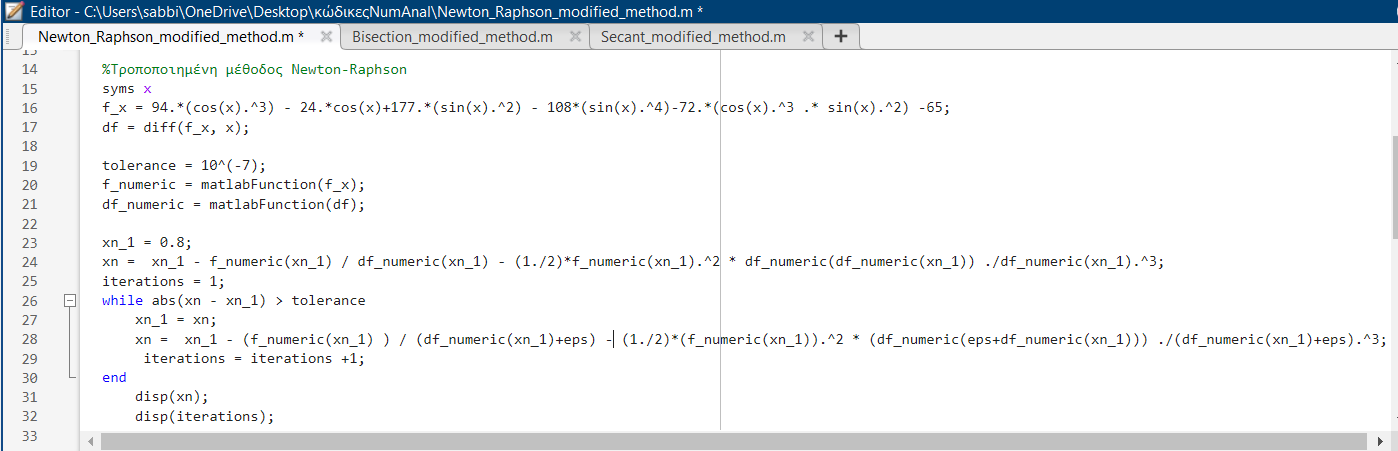
\includegraphics[width=0.9\textwidth,height=0.3\textheight]{SecantModified.png} 


    \vspace{0.5cm} 
    
    
    \small\textit{Note: The above code was implemented without the assistance of language model.}
\end{tcolorbox}

\subsection{Comparison of Modified methods with the initial methods}

After experimenting 100 times for each initial method and its corresponding modified,for a variety of different initializations the results upon the convergence speed are the following based on an avarage value of iterations:
\begin{tcolorbox}[colback=blue!10, colframe=gray!80, width=\textwidth, sharp corners]
    \centering
    \begin{tabular}{|l|c|}
        \hline
        \textbf{Method} & \textbf{Average Iteration Speed} \\ \hline
        Bisection Method & 20.51 \\ \hline
        Modified Bisection Method & 19.79 \\ \hline
        \multicolumn{2}{|c|}{} \\ \hline 
        Newton-Raphson Method & 19.29\\ \hline
        Modified Newton-Raphson Method & 19.51 \\ \hline
        \multicolumn{2}{|c|}{} \\ \hline
        Secant Method & 39.85\\ \hline
        Modified Secant Method & 18.67 \\ \hline
    \end{tabular}

    \vspace{0.5cm}

    \small\textit{Note: Convergence speed comparison : Initial methods vs Modified methods}
\end{tcolorbox}



\begin{tcolorbox}[colback=gray!10, colframe=gray!80, width=\textwidth, sharp corners]
    \centering 
    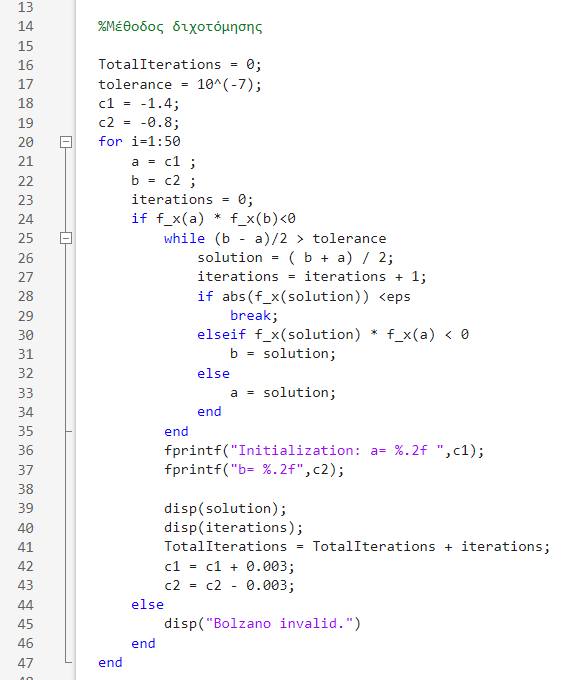
\includegraphics[width=0.8\textwidth,height=0.3\textheight]{Experiment100Times1.png} 
    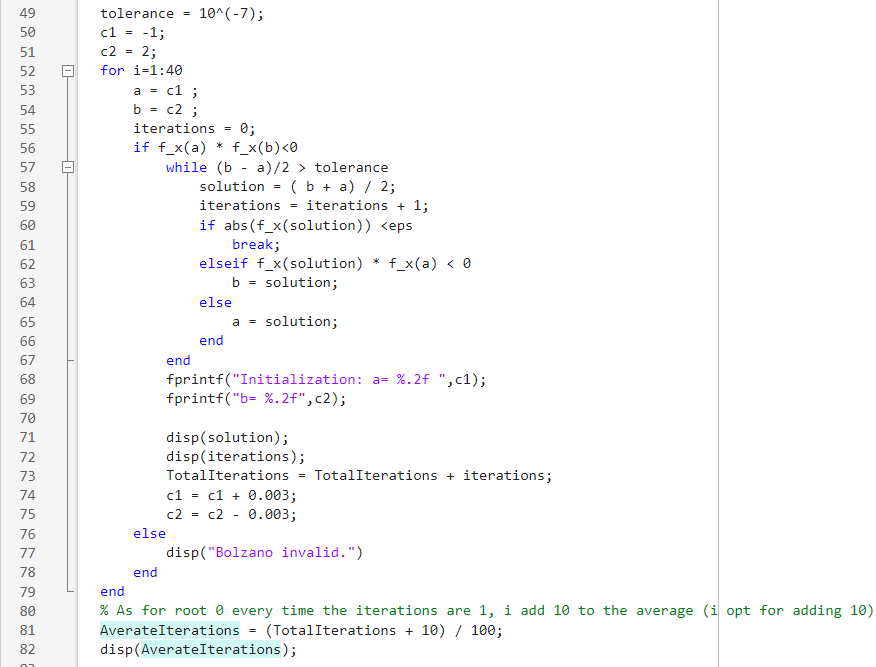
\includegraphics[width=0.8\textwidth,height=0.3\textheight]{Experiment100Times2.png} 


    \vspace{0.5cm} 
   
    
    \small\textit{Note: Code for testing Bisection method 100 times and finding an average iteration speed.}
\end{tcolorbox}

\begin{tcolorbox}[colback=gray!10, colframe=gray!80, width=\textwidth, sharp corners]
    \centering 
    


    \vspace{0.6cm} 
    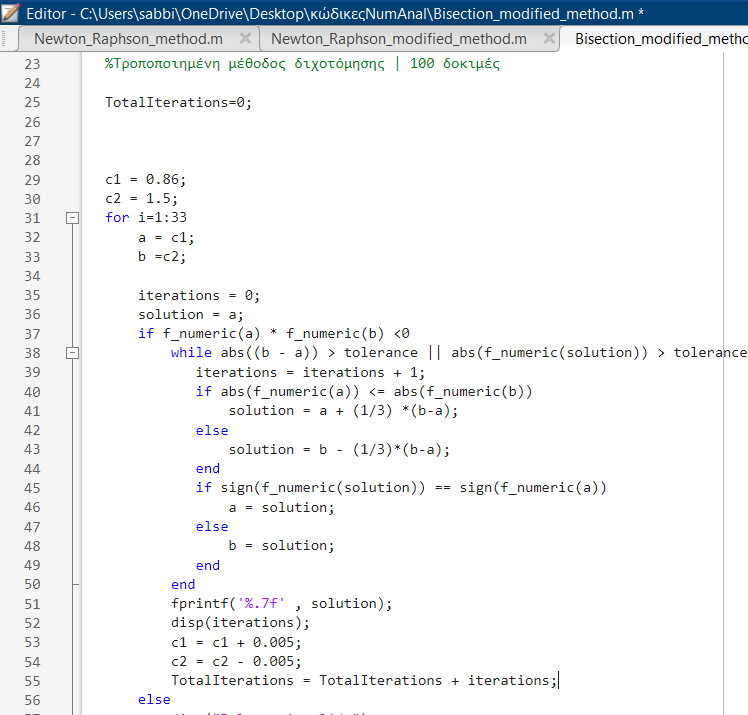
\includegraphics[width=0.8\textwidth,height=0.3\textheight]{ExpModifiedBisection100Times1.png} 
    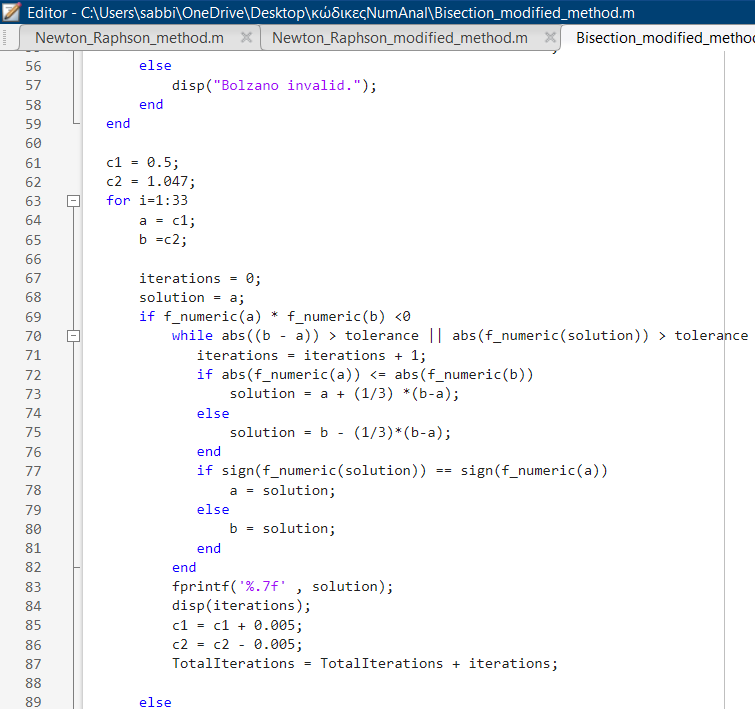
\includegraphics[width=0.8\textwidth,height=0.3\textheight]{ExpModifiedBisection100Times2.png.png}
    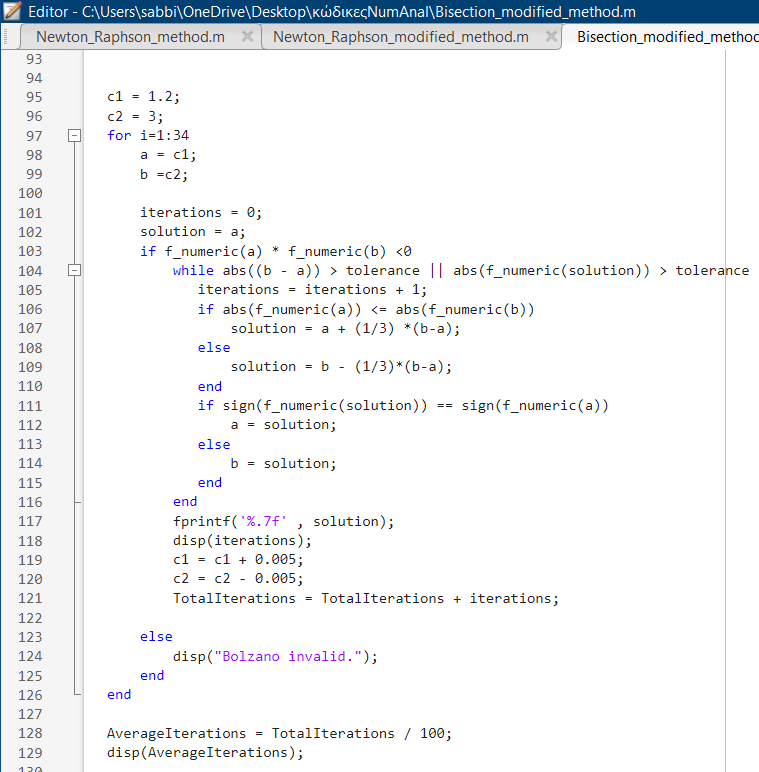
\includegraphics[width=0.8\textwidth,height=0.3\textheight]{ExpModifiedBisection100Times3.png.png}
    
    
    \small\textit{Note: Code for testing  modified Bisection method 100 times and finding an average iteration speed.}
\end{tcolorbox}

\begin{tcolorbox}[colback=gray!10, colframe=gray!80, width=\textwidth, sharp corners]
    \centering 
   
    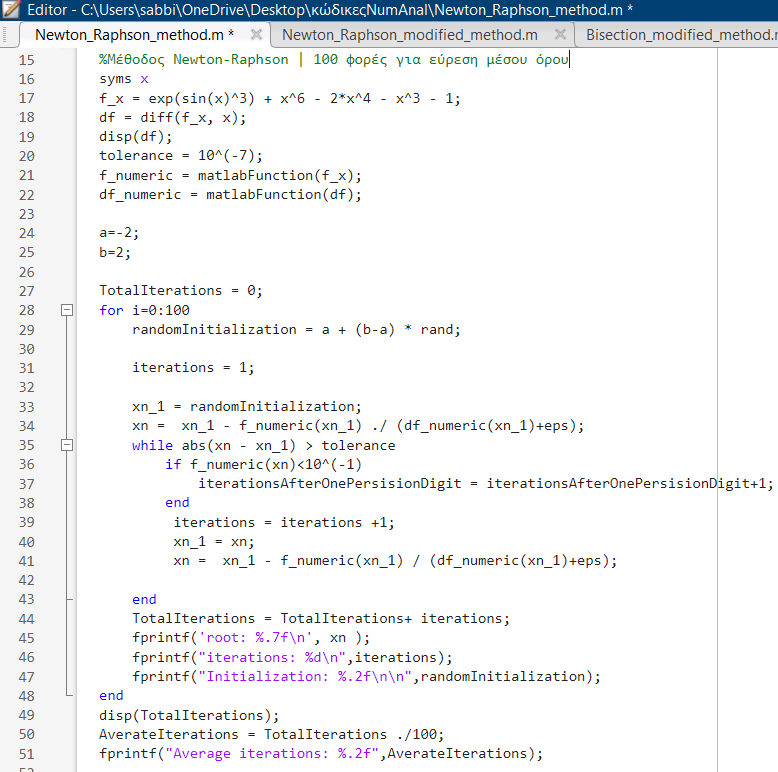
\includegraphics[width=0.8\textwidth,height=0.4\textheight]{NewtonRaphson100Times.png} 
      
    \small\textit{Note: Code for testing Newton Raphson method 100 times to test the average convergence speed.}
\end{tcolorbox}

\begin{tcolorbox}[colback=gray!10, colframe=gray!80, width=\textwidth, sharp corners]
    \centering 
   
    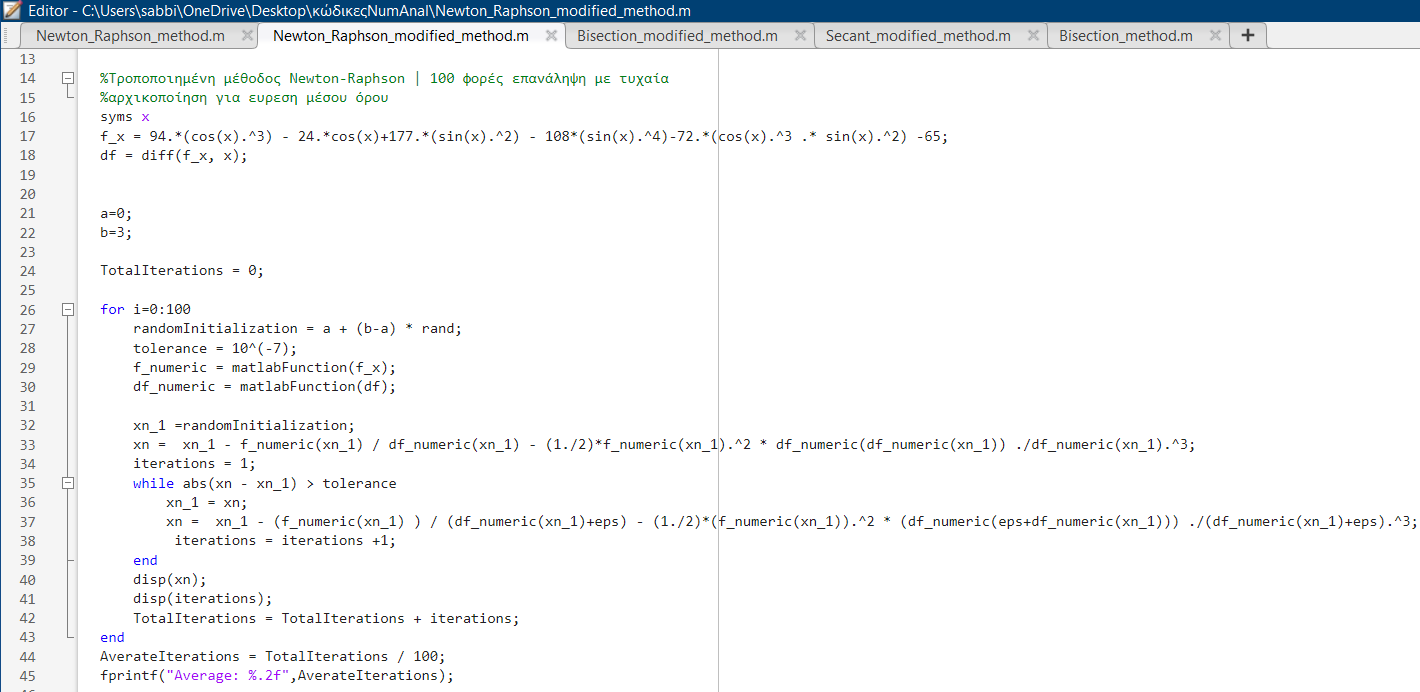
\includegraphics[width=0.9\textwidth,height=0.3\textheight]{ModifiedNR100Times.png} 
      
    \small\textit{Note: Code for testing modified Newton-Raphson method 100 times to test the average convergence speed.}
\end{tcolorbox}

\begin{tcolorbox}[colback=gray!10, colframe=gray!80, width=\textwidth, sharp corners]
    \centering 
   
    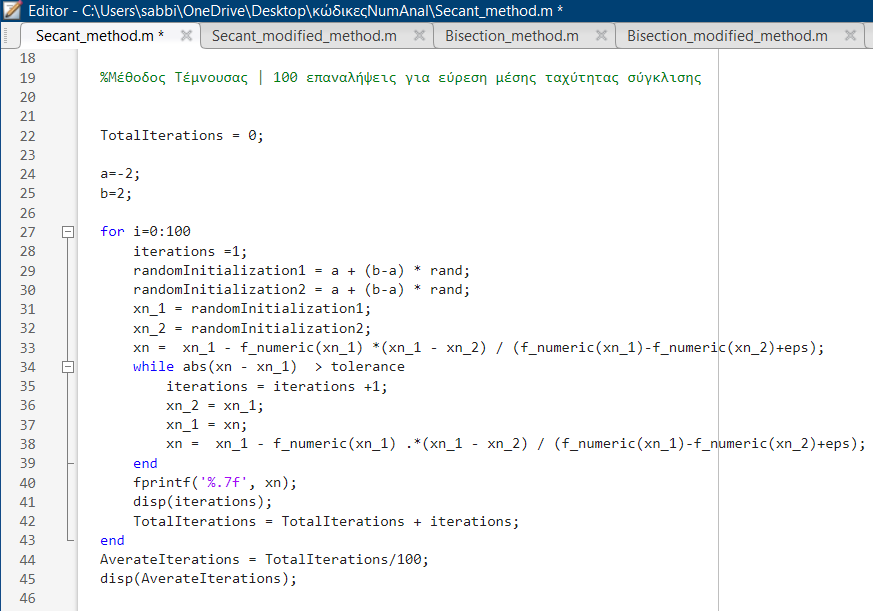
\includegraphics[width=0.8\textwidth,height=0.3\textheight]{Secant100Times.png} 
      
    \small\textit{Note: Code for testing Secant method 100 times to test the average convergence speed.}
\end{tcolorbox}

\begin{tcolorbox}[colback=gray!10, colframe=gray!80, width=\textwidth, sharp corners]
    \centering 
    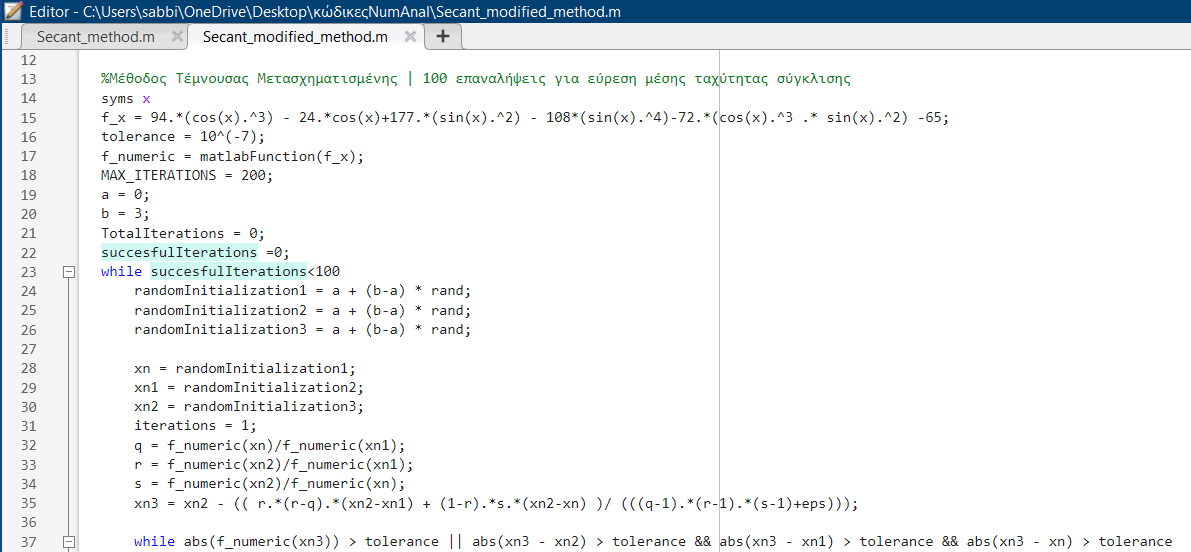
\includegraphics[width=0.9\textwidth,height=0.3\textheight]{ModifiedSecant100Times1.png} 
    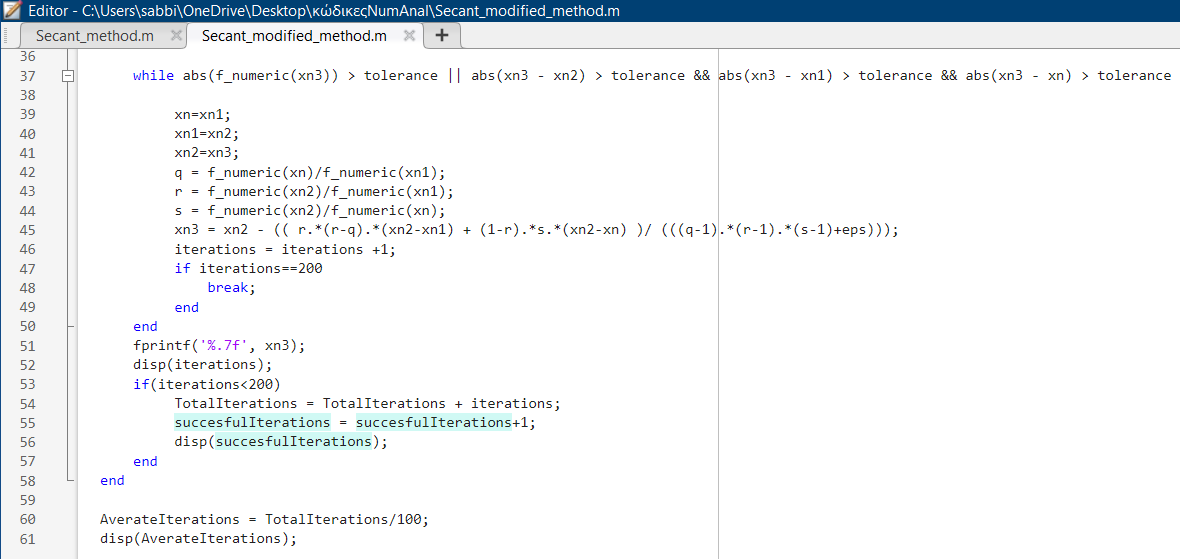
\includegraphics[width=0.85\textwidth,height=0.3\textheight]{ModifiedSecant100Times2.png} 

    \vspace{0.5cm} 
    
    \small\textit{Note: Code for testing modified Secant method 100 times to test the average convergence speed.}
\end{tcolorbox}

\newpage
\section{Exercise 3}
\subsection{LU decomposition}
After writing the initial code that is displayed below, the only problem that occurred during the LU Decomposition was that the L Matrix was created but with its elements not being placed in the correct positions.
Passing the code through Chat GPT, lead to the final code also being displayed below. The main changes conducted by GPT were:
\begin{enumerate}
    \item the L Matrix updating
    \item the partial pivoting implementation for the changing of the rows based on the $max$ element.
    
\end{enumerate}
\begin{tcolorbox}[colback=gray!10, colframe=gray!80, sharp corners]
    \centering
    \begin{minipage}[t]{0.48\textwidth}
        \centering
        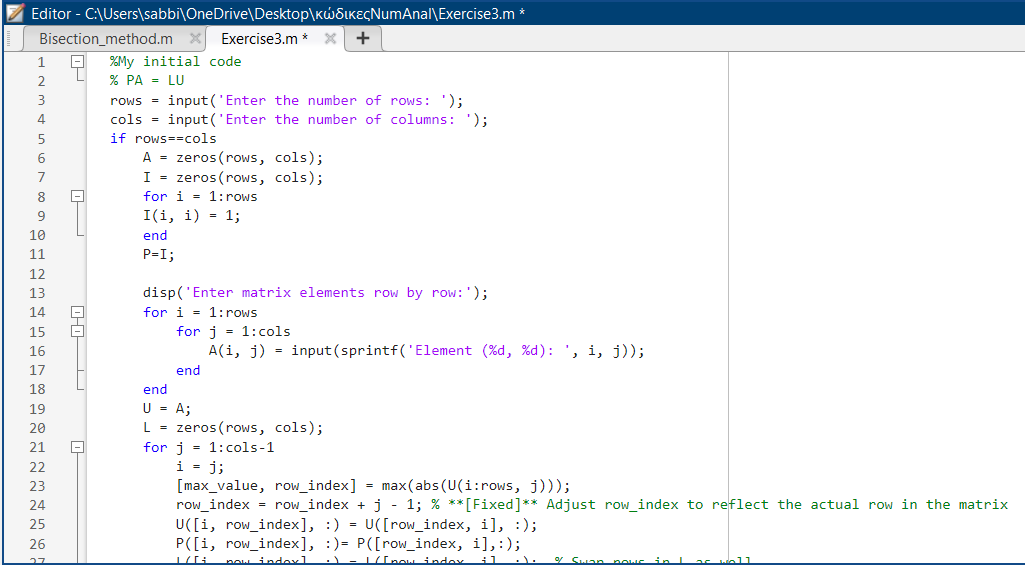
\includegraphics[width=\textwidth, height=0.25\textheight]{PALU1.png}
    \end{minipage}
    \hfill
    \begin{minipage}[t]{0.48\textwidth}
        \centering
        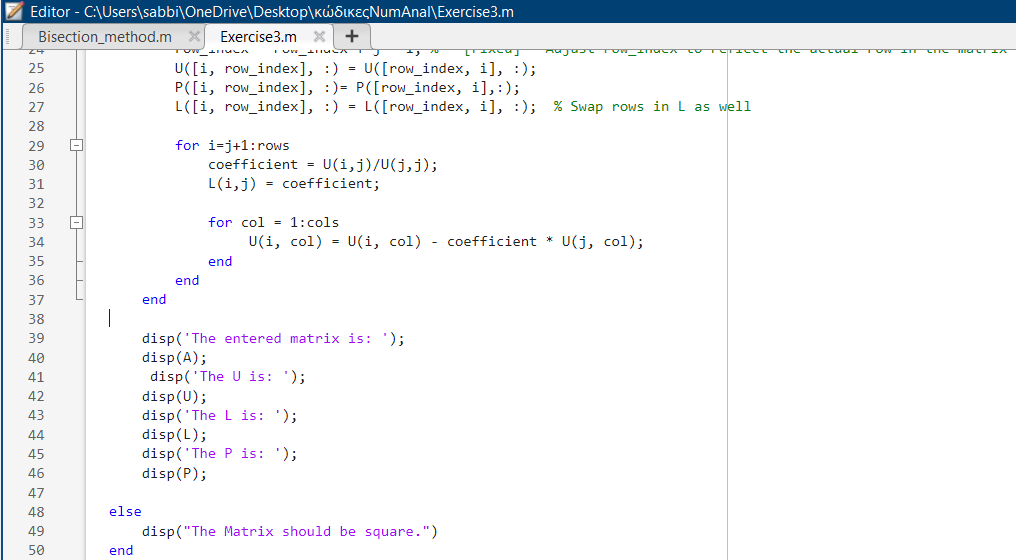
\includegraphics[width=\textwidth, height=0.25\textheight]{PALU2.png}
    \end{minipage}

    \vspace{0.5cm}
    
    \small\textit{Note: The initial code.}
\end{tcolorbox}

\begin{tcolorbox}[colback=gray!10, colframe=gray!80, width=\textwidth, sharp corners]
    \centering 
    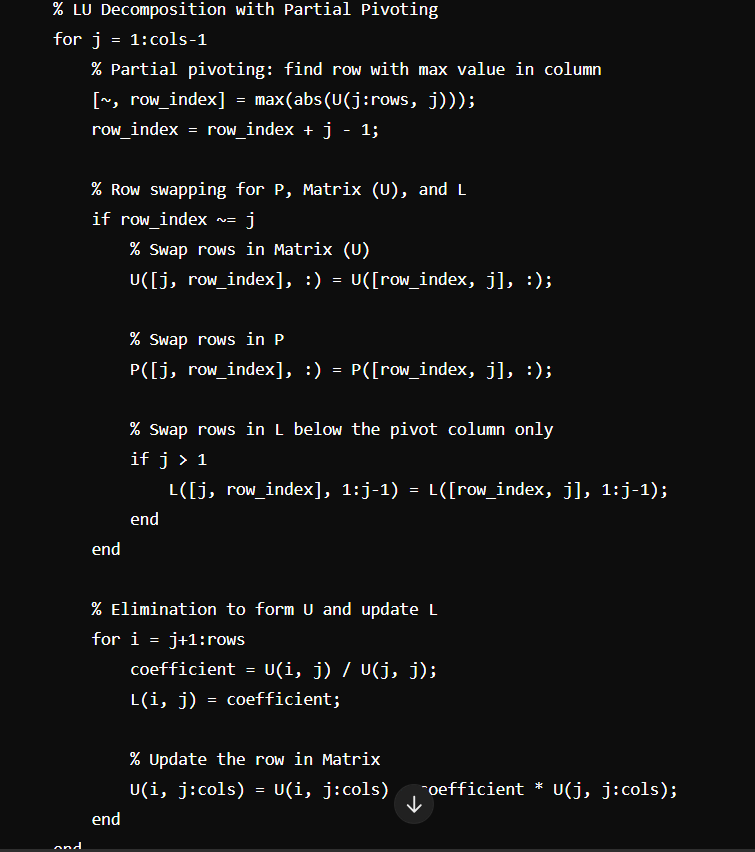
\includegraphics[width=0.9\textwidth,height=0.6\textheight]{PALUGPT.png} 
    

    \vspace{0.5cm} 
    
    \small\textit{Note: Final code, after Chat GPT's changes to the initial one.}
\end{tcolorbox}

After finding the $PA=LU$ decomposition and having to solve the equation $Ax= b$
the following is true:
\begin{center}
    $Ax = b$\\
    $PAx = Pb$\\
   $ LUx = Pb$\\
\end{center}
First, considering that $Ly=Pb$  $y = L \ Pb;$ in Matlab code, forward substitution is used for solving, as Matlab documentation suggests.
Then what remains is to consider $Ux=y$ and solve it using back substitution with the Matlab code $x = U \ y;$
The code is displayed below:

\begin{tcolorbox}[colback=gray!10, colframe=gray!80, width=\textwidth, sharp corners]
    \centering 
    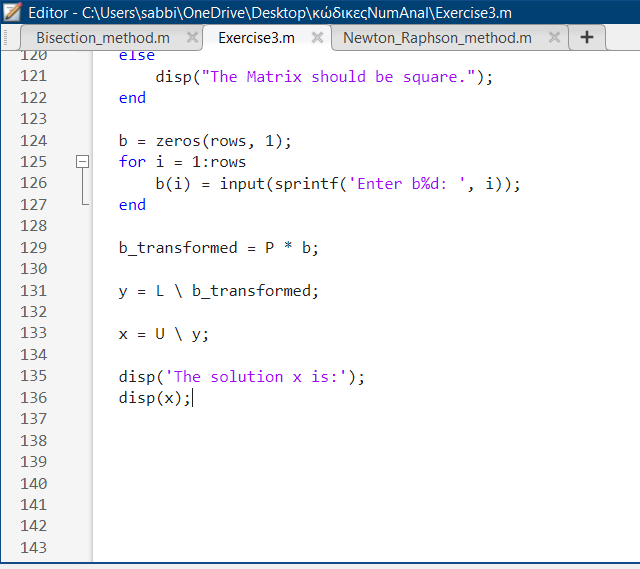
\includegraphics[width=0.9\textwidth,height=0.4\textheight]{Ex3SolvingEquation.png} 
    

    \vspace{0.2cm} 
    
    \small\textit{Note: The code was created using no language model , but Matlab documentation.}
\end{tcolorbox}



\subsection{Cholesky}
For the Cholesky function, Chat GPT was used in order to find the Equation that produces the L matrix. The code implemented was based on the answers that are displayed below.

\begin{tcolorbox}[colback=gray!10, colframe=gray!80, width=\textwidth, sharp corners]
    \centering 
    
\includegraphics[width=0.9\textwidth,height=0.1\textheight]{CholeskyGPT1.png} 
    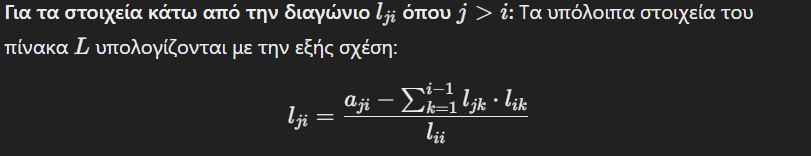
\includegraphics[width=0.9\textwidth,height=0.1\textheight]{CholeskyGPT2.png} 
    

    \vspace{0.2cm} 
    
    \small\textit{Note: The equations were provided using Chat GPT.}
\end{tcolorbox}

\begin{tcolorbox}[colback=gray!10, colframe=gray!80, width=\textwidth, sharp corners]
    \centering 
    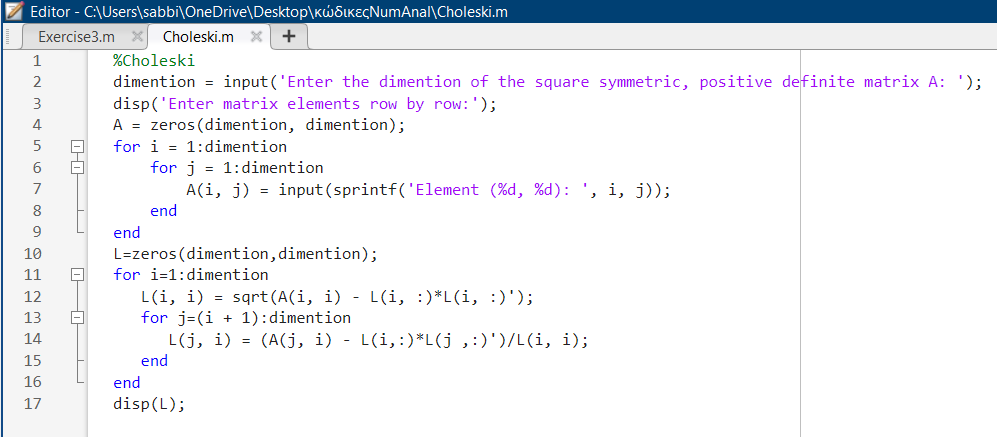
\includegraphics[width=0.9\textwidth,height=0.26\textheight]{Cholesky.png}     

    \vspace{0.2cm} 
    
    \small\textit{Note:No language model was used to implement the code itself except the equations.}
\end{tcolorbox}
\subsection{Gauss-Seidel}
The Gauss-Seidel method for the given system, both for $n = 10$ and for $n=5000$
produces the solution $x=(1,1,1,...,1)$.
\begin{tcolorbox}[colback=gray!10, colframe=gray!80, width=\textwidth, sharp corners]
    \centering 
    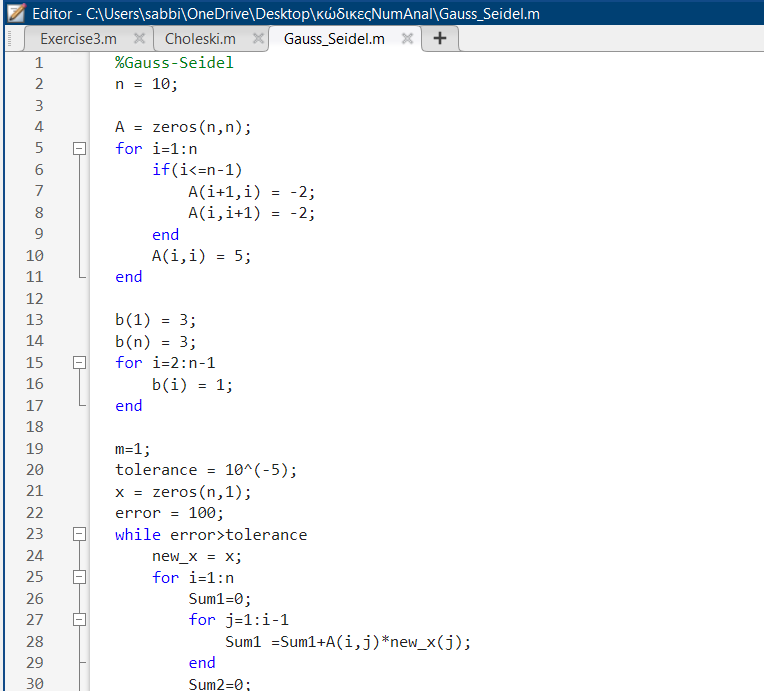
\includegraphics[width=0.9\textwidth,height=0.231\textheight]{Gauss_Seidel1.png} 
    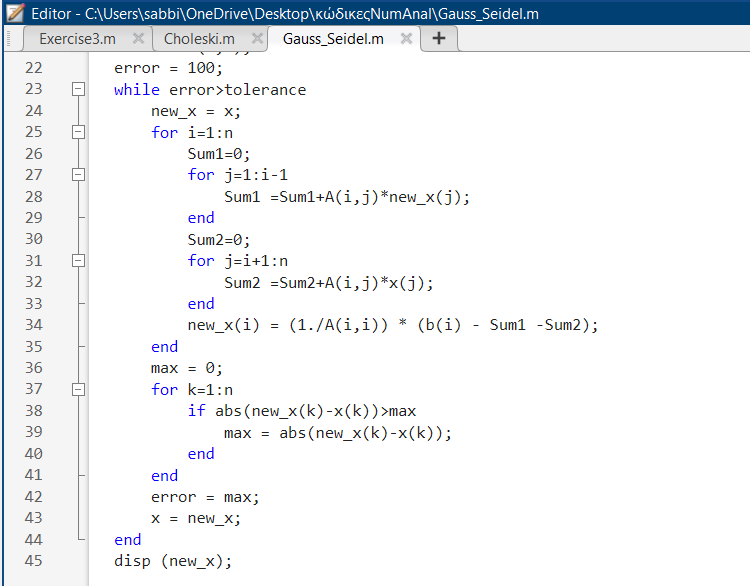
\includegraphics[width=0.9\textwidth,height=0.231\textheight]{Gauss_Seidel2.png}     


    \vspace{0.2cm} 
    
    \small\textit{Note:The above code was created without the assistance of a language model.}
\end{tcolorbox}


\section{Exercise 4}
\subsection{Stochastic G Matrix}
In order for $G$ to be a stochastic matrix, each of each columns should have a summary of 1 (its maximum eigenvalue should be equal to 1).
Each of  G matrix's element is given as follows.
\begin{center}
\begin{equation*}      
       G(i,j)=\frac{q}{n} + \frac{A(j,i)(1-q)}{n_i}
\end{equation*}

\end{center}

For each $i$ from 1 to $n$, the following relationship must be true:


\begin{align*}
\sum_{i=1}^{n} \left( \frac{q}{n} + \frac{A(j,i)(1-q)}{n_j} \right) &= 1 \\
\iff n \cdot\frac{q}{n} + \sum_{i=1}^{n}\left(\frac{A(j,i)(1-q)}{n_j} \right) &= 1 \\
\iff \sum_{i=1}^{n} \left(\frac{A(j,i)(1-q)}{n_j} \right) &= 1 - q \\
\iff \sum_{i=1}^{n} \left(\frac{A(j,i)}{n_j} \right) &= 1 \\
\iff \frac{\sum_{i=1}^{n} A(j,i)}{n_j} &= 1
\end{align*}

Which is indeed true, as for i from 1 to n, $\sum_{i=1}^{n} A(j,i)$ gives the summary of the column $j$, which is equal to $n_j$.
\newpage
\subsection{Creation of G}


The vertex that corresponds to the eigenvector of the maximum eigenvalue is:

\[
\mathbf{p} = \left( 
0.0268246, 0.0298611, 0.0298611, 0.0268246, 0.0395872, 0.0395872, 0.0395872, 0.0395872, 
\right.
\]
\[
\left.
0.0745644, 0.1063200, 0.1063200, 0.0745644, 0.1250916, 0.1163279, 0.1250916 
\right)
\]

\begin{tcolorbox}[colback=gray!10, colframe=gray!80, width=\textwidth, sharp corners]
    \centering 
    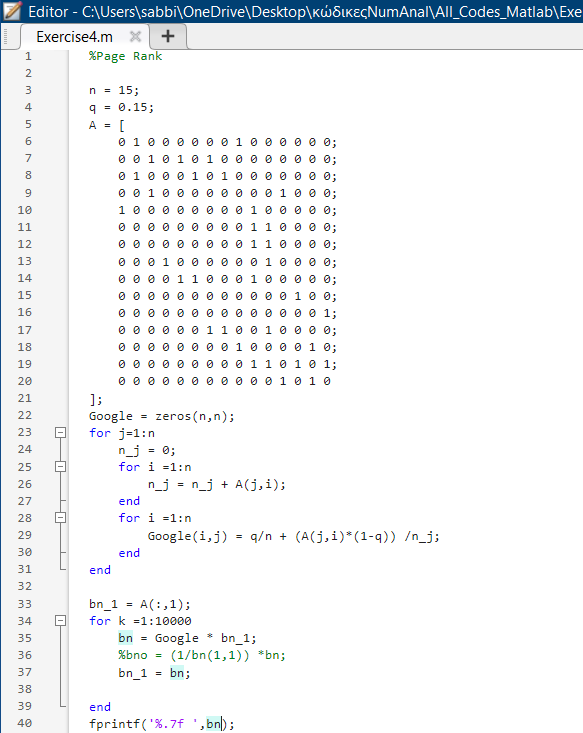
\includegraphics[width=0.6\textwidth,height=0.5\textheight]{PageRank.png}     

    \vspace{0.2cm} 
    
    \small\textit{Note:The code implementing the G matrix and the vertex that corresponds to the eigenvector of the maximum eigenvalue. No language model was used.}
\end{tcolorbox}

\subsection{Adding edges}
Having in mind that the needed page rank to be increased is that of \textbf{page 6}
after \textbf{adding} the edges:
\[
10 \to 6, \quad 11 \to 6, \quad 13 \to 6, \quad 14 \to 6,
\]
and \textbf{removing} the already existing edge:
\[
9 \to 5,
\]
the result is as follows:
The page rank of page 6 is \textbf{increased} from \textbf{0.0395872 to 0.1945922}
That happens because the 4 new edges that lead to page 6 are beginning from pages that already have an increased page rank compared to the other pages. Also the removed edge is not directly affecting the page rank of page 6 so it is preferred for its irrelevancy. 

\begin{tcolorbox}[colback=gray!10, colframe=gray!80, width=\textwidth, sharp corners]
    \centering 
    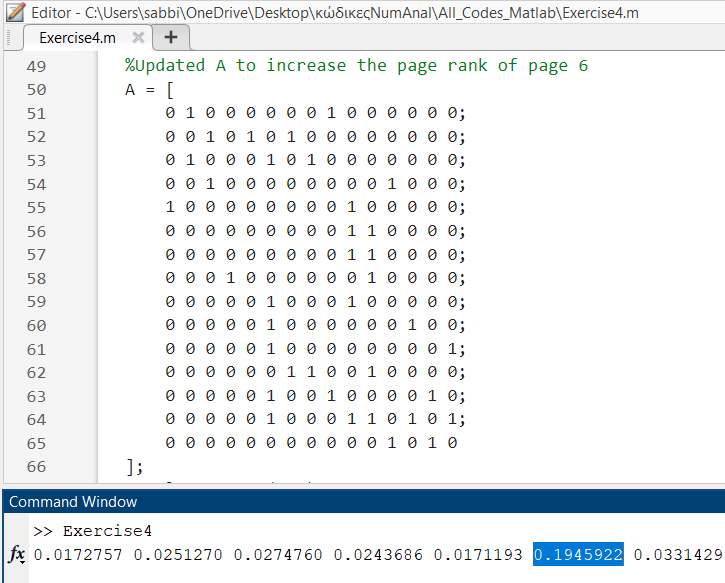
\includegraphics[width=0.6\textwidth,height=0.33\textheight]{Page6increase.png}     

    \vspace{0.2cm} 
    
    \small\textit{Note: Code displaying updated matrix A targeting to increase the page rank of page 6}
\end{tcolorbox}

\subsection{Experimenting with q}
\begin{itemize}
  
\item After \textbf{decreasing q} to 0.02 in the new Graph the page rank of page 6 that was previously increased now seems to be \textbf{increased}  even more from 0.1945922 to 0.2279782.
\item Also \textbf{increasing q} to 0.6 \textbf{decreases the page rank of page 6} from 0.1945922 to 0.1126697.
\end{itemize}
It is evident that when the \textbf{q variable is notably increased}, being the probability of a user moving to a random page , that means that \textbf{it is more likely for a user to move to a random page} which leads to the connection - references - edges between pages playing a less important role. The opposite is happening when \textbf{q is decreased} , meaning that a user is not likely to move to random pages but \textbf{very much likely to move to pages referenced in the page he is already in}. That is the reason that page 6 page rank is notably increased when q has a small value: because many other pages with high page ranks are pointing - including a reference to page 6.

\subsection{Page 11 tries to increase its page rank}\
The result shows that the page rank of page 11 \textbf{is increased from 0.1063200 to 0.1240084} which indicates that 
the strategy of changing the strength of  $A(12,11)$ and $A(8,11)$ links to page 11 is indeed working. 
\begin{tcolorbox}[colback=gray!10, colframe=gray!80, width=\textwidth, sharp corners]
    \centering 
    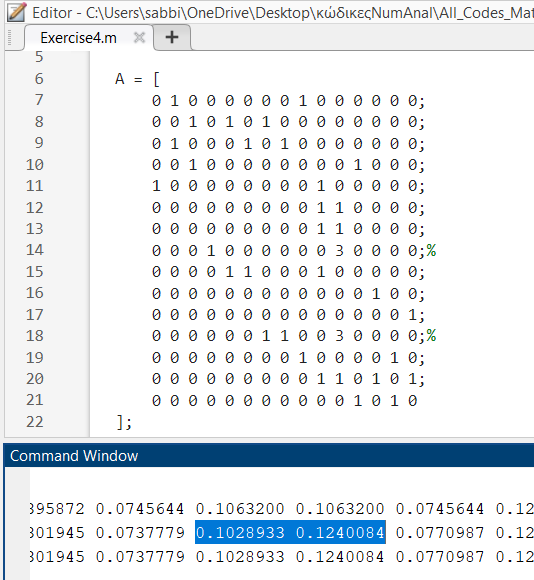
\includegraphics[width=0.6\textwidth,height=0.33\textheight]{Ex4Put3.png}     

    \vspace{0.2cm} 
    
    \small\textit{Note: Code displaying updated matrix A targeting to increase the page rank of page 11 by changing the strength at which pages 8 and 12 point at it.}
\end{tcolorbox}
\vspace{0.3cm}
\subsection{Deletion of page 10}
\vspace{0.3cm}

\begin{tabular}{|c|c|c|c|}
\hline
\textbf{Page} & \textbf{Initial Page Rank} & Page Rank After Deletion & \textbf{Change} \\
\hline
Page 1 & 0.0268246 & 0.0470950 & \textbf{↑ Increase} \\
\hline
Page 2 & 0.0298611 & 0.0409114 & \textbf{↑ Increase} \\
\hline
Page 3 & 0.0298611 & 0.0359356 & \textbf{↑ Increase} \\
\hline
Page 4 & 0.0268246 & 0.0320700 & \textbf{↑ Increase} \\
\hline
Page 5 & 0.0395872 & 0.0428008 & \textbf{↑ Increase} \\
\hline
Page 6 & 0.0395872 & 0.0413910 & \textbf{↑ Increase} \\
\hline
Page 7 & 0.0395872 & 0.0516587 & \textbf{↑ Increase} \\
\hline
Page 8 & 0.0395872 & 0.0502489 & \textbf{↑ Increase} \\
\hline
Page 9 & 0.0745644 & 0.0482235 & \textbf{↓ Decrease} \\
\hline
Page 10 & 0.1063200 & - & - \\
\hline
Page 11 & 0.1063200 & 0.1709627 & \textbf{↑ Increase} \\
\hline
Page 12 & 0.0745644 & 0.1035981 & \textbf{↑ Increase} \\
\hline
Page 13 & 0.1250916 & 0.0411619 & \textbf{↓ Decrease} \\
\hline
Page 14 & 0.1163279 & 0.1074622 & \textbf{↓ Decrease} \\
\hline
Page 15 & 0.1250916 & 0.1864802 & \textbf{↑ Increase} \\
\hline
\end{tabular}


\end{document}



